% !TEX TS-program = pdflatex
% !TEX encoding = UTF-8 Unicode

% This is a simple template for a LaTeX document using the "article" class.
% See "book", "report", "letter" for other types of document.

\documentclass[11pt]{article} % use larger type; default would be 10pt

\usepackage[utf8]{inputenc} % set input encoding (not needed with XeLaTeX)

%%% Examples of Article customizations
% These packages are optional, depending whether you want the features they provide.
% See the LaTeX Companion or other references for full information.

%%% PAGE DIMENSIONS
\usepackage{geometry} % to change the page dimensions
\geometry{letterpaper} % or letterpaper (US) or a5paper or....
% \geometry{margin=2in} % for example, change the margins to 2 inches all round
% \geometry{landscape} % set up the page for landscape
%   read geometry.pdf for detailed page layout information

\usepackage{graphicx} % support the \includegraphics command and options
\usepackage{grffile}

% \usepackage[parfill]{parskip} % Activate to begin paragraphs with an empty line rather than an indent

%%% PACKAGES
\usepackage{booktabs} % for much better looking tables
\usepackage{array} % for better arrays (eg matrices) in maths
\usepackage{paralist} % very flexible & customisable lists (eg. enumerate/itemize, etc.)
\usepackage{verbatim} % adds environment for commenting out blocks of text & for better verbatim
\usepackage{subfig} % make it possible to include more than one captioned figure/table in a single float
% These packages are all incorporated in the memoir class to one degree or another...

\usepackage{hyperref}

%%% HEADERS & FOOTERS
\usepackage{fancyhdr} % This should be set AFTER setting up the page geometry
\pagestyle{fancy} % options: empty , plain , fancy
\renewcommand{\headrulewidth}{0pt} % customise the layout...
\lhead{}\chead{}\rhead{}
\lfoot{}\cfoot{\thepage}\rfoot{}

%%% SECTION TITLE APPEARANCE
\usepackage{sectsty}
\allsectionsfont{\sffamily\mdseries\upshape} % (See the fntguide.pdf for font help)
% (This matches ConTeXt defaults)

%%% ToC (table of contents) APPEARANCE
\usepackage[nottoc,notlof,notlot]{tocbibind} % Put the bibliography in the ToC
\usepackage[titles,subfigure]{tocloft} % Alter the style of the Table of Contents
\renewcommand{\cftsecfont}{\rmfamily\mdseries\upshape}
\renewcommand{\cftsecpagefont}{\rmfamily\mdseries\upshape} % No bold!

%%% END Article customizations

%%% The "real" document content comes below...

\title{Accessing the Daly Lab DB}
\author{Brandon Avila}
%\date{} % Activate to display a given date or no date (if empty),
         % otherwise the current date is printed 


\begin{document}
\maketitle
\abstract{This document describes how to access and use Daly Lab database, created on Sept. 19, 2016. The date at the top should reflect the most recent change to this document.}

\section{Introduction}
The database is set up through the Broad's database services. It is stored and backed up on the internal filesystems, and can be accessed without the explicit location with a connect string given later in this document.

The purpose of this DB is to store relevant information to link samples, projects, cohorts, phenotype files, etc. in a central, easy to access location. With this, we should be able to generate summaries, browse the data, and batch-upload new information without bothering Christine for everything we need.

\section{User Access}
There are two pieces of information you will need to access the database with any given client. The first is the connect string:
\begin{verbatim}
BRDPDB01 =
    (DESCRIPTION =
        (ADDRESS = (PROTOCOL = TCP)(HOST = oracon-1)(PORT = 1521))
        (CONNECT_DATA  =
            (SERVICE_NAME = brdpdb01)
        )
    )
\end{verbatim}
This tells your client where to find the DB and how to connect to it.

The second thing you'll need is the login credentials, or \emph{user}. At the moment, there is only one user that has every permission except creating new users. I will see about talking to the DBA to make seperate read and write users so nobody accidentally \texttt{DROP}s a \texttt{TABLE}. The user with all permissions is the following:
\begin{verbatim}
user: dlab_samples
pass: [redacted] email me for password, since this file is now on github
\end{verbatim}

\section{Oracle SQL Developer}
If you already have a preferred client, you don't need this, but if you've never directly accessed a DB before, this is a good tool to start with. It's possible that in a while, BITS will begin supporting a browser based client that will look a lot snazzier than this, but this is what we have for now.

First, you should download the latest version of JDK at \url{http://www.oracle.com/technetwork/java/javase/downloads/jdk8-downloads-2133151.html}. Then, you can get the actual client at \url{http://www.oracle.com/technetwork/developer-tools/sql-developer/downloads/index.html}. The download should be pretty straightforward.

From here, you should open it up, and immediately set the \texttt{tnsnames} path. To do this, go to \texttt{Oracle SQL Developer --> Preferences...} in the file menu. Navigate to the Advanced category under Database, and change the Tnsnames Directory as shown below.
\\
\\
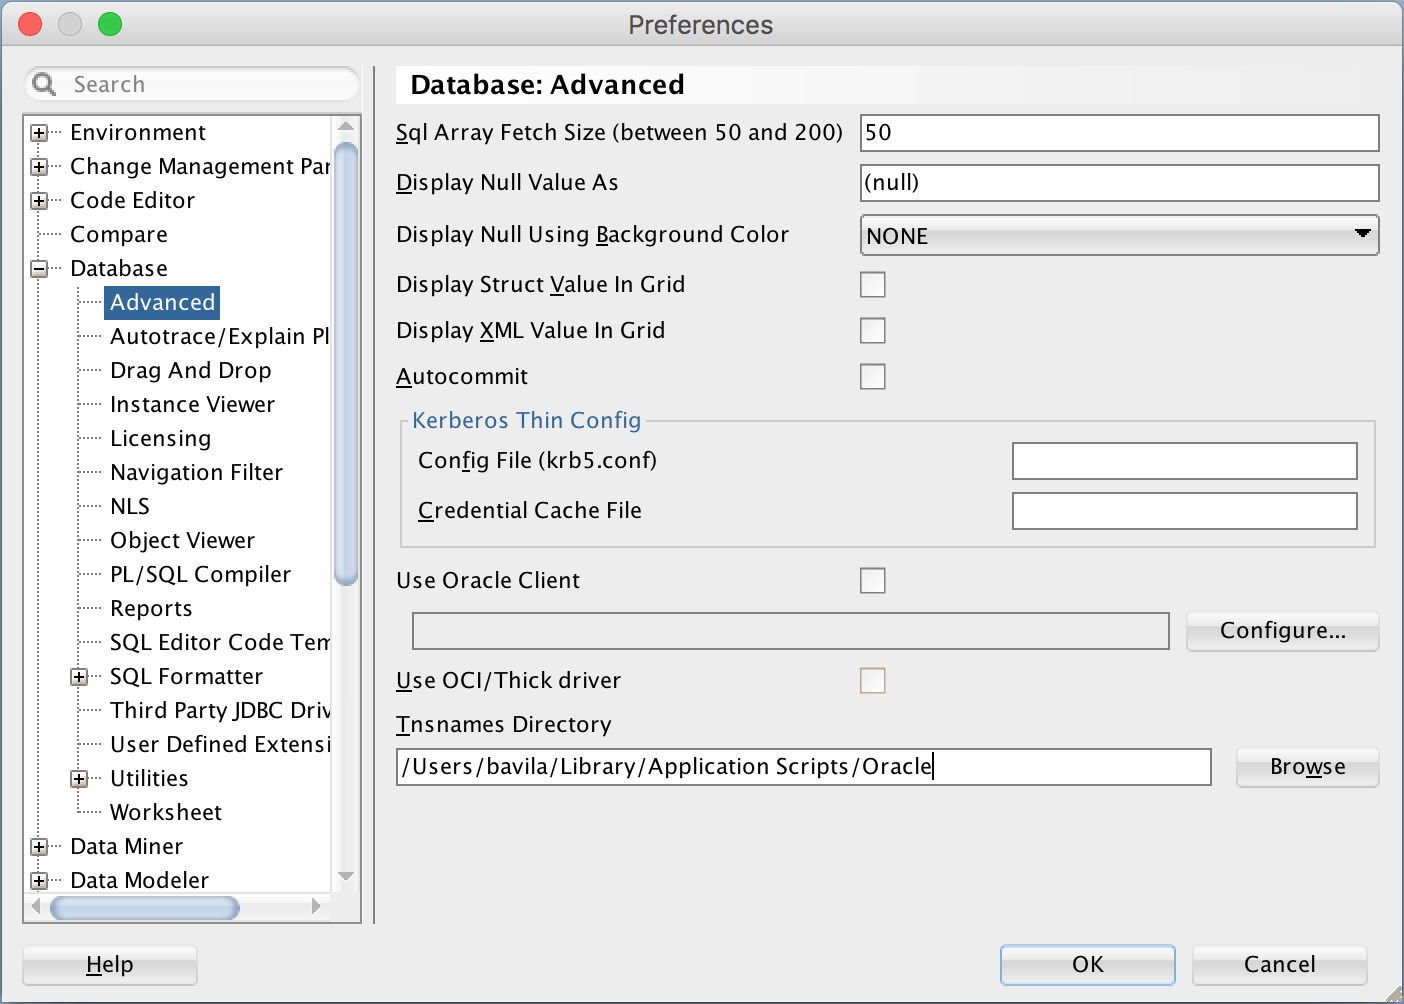
\includegraphics[scale=0.5]{TNS Preferences.png}
\\
\\
It doesn't matter where you set it, but make it some place you can easily access.

Next, go into the directory you just set, and create a file named \texttt{tnsnames.ora} containing the connect string listed above.

Now you should be able to connect. To set up the connection, click the appropriate button on the Connections panel to the left. Set the preferences as shown here:
\\
\\
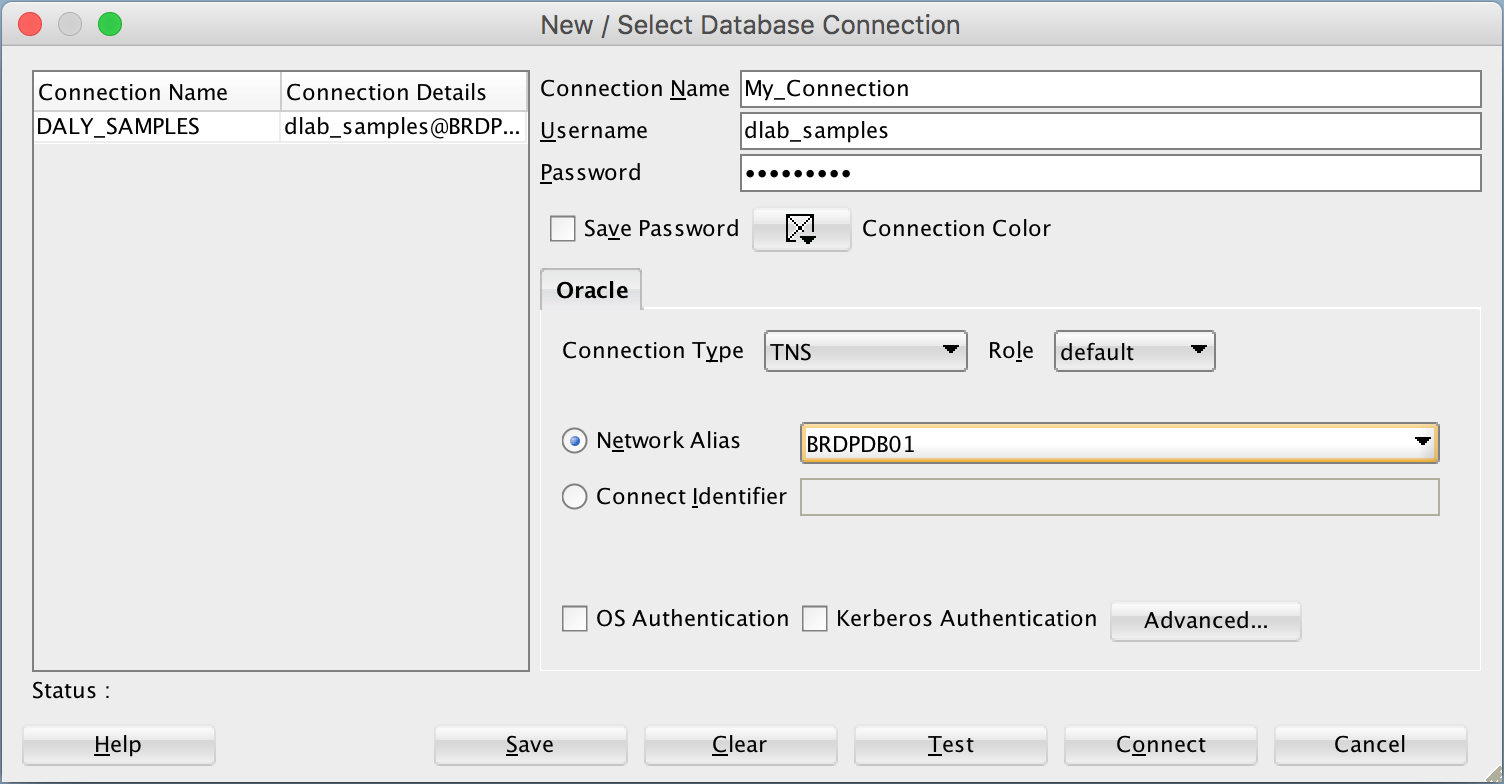
\includegraphics[scale=0.5]{Connection.png}
\\
\\
You can name the connection whatever you want, but the username and password should be those written above. Make sure the Connection Type is set to TNS and the Role is set to default. Select the Network Alias \texttt{BRDPDB01} from the dropdown menu. Use the Test button to make sure the connection is set up right, then click Connect. From now on, the connection should appear on the Connections panel whenever you open SQL Developer. You may have to manually connect by right-clicking and selecting connect or something.

This client contains a bunch of features, but if you just want to see the data in a spreadsheet-like format, you can drag a table in the DB from the Connections panel to the main panel. The worksheets can be used to write SQL statements, and there exists a graphical query builder that I haven't really figured out yet.

For more info on this tool, you can check out the documentation at \url{http://docs.oracle.com/cd/E12151_01/}.

\section{Other Tools}
So far, I've pretty successfully been using the cx\_Oracle Python library to access the DB from the command line. The package is availabel at \url{https://pypi.python.org/pypi/cx_Oracle/5.2.1}, and the link to the documentation is \url{https://cx-oracle.readthedocs.io/en/latest/}. I can send a sample script if necessary, but it should be pretty easy to figure out how to add this into your pipeline.


\end{document}
